\documentclass[12pt]{article}
\usepackage[catalan]{babel}
\usepackage[utf8]{inputenc}
\usepackage{listings}
\usepackage{color}
\usepackage{graphicx}
\usepackage{verbatim}
\usepackage[obeyspaces]{url}
\usepackage{appendix}
\usepackage{dirtytalk}

\definecolor{codegreen}{rgb}{0,0.6,0}
\definecolor{codegray}{rgb}{0.5,0.5,0.5}
\definecolor{codepurple}{rgb}{0.58,0,0.82}
\definecolor{backcolour}{rgb}{0.95,0.95,0.92}
 
\lstset{
	backgroundcolor=\color{backcolour},   
	breaklines=true, 
	numbers=left,
	basicstyle=\footnotesize,
	backgroundcolor=\color{backcolour},   
    commentstyle=\color{codegreen},
    keywordstyle=\color{magenta},
    numberstyle=\tiny\color{codegray},
    stringstyle=\color{codepurple},
    basicstyle=\footnotesize,
    breakatwhitespace=false,         
    breaklines=true,                 
    captionpos=b,                    
    keepspaces=true,                 
    numbers=left,                    
    numbersep=5pt,                  
    showspaces=false,                
    showstringspaces=false,
    showtabs=false,                  
    tabsize=2
}
\setlength{\parindent}{0pt}

\begin{document}
\begin{titlepage}
		\centering
		
\includegraphics[width=0.5\textwidth]{imatges/logo.png}\par\vspace{1cm}
		{\huge\bfseries Projecte final\par}
		\vspace{1cm}
		{\scshape\Large Màster en enginyeria informàtica\par}
		\vspace{1.5cm}
		{\Large\itshape Oscar Galera i Alfaro\par}
		\vspace{1cm}
		{\Large\itshape Disseny i implementació de xarxes i sistemes distribuïts\par}
		\vspace{2cm}
		\vfill
		\vfill
		{\large \today\par}
\end{titlepage}
\clearpage
\tableofcontents
\clearpage
\listoffigures

%%%%%%%%%%%%%DEFINICIÓ DEL PROBLEMA%%%%%%%%%%%%
\clearpage
\section{Problema\label{problema}}
El problema a resoldre, és l'obtenció del posicionament i tipologia de sensors (respectant un cost màxim) en una xarxa de distribució d'aigua. 
\\\\La finalitat d'aquesta simulació és controlar la qualitat de l'aigua maximitzant la informació proporcionada per aquests sensors amb el mínim cost possible.

\subsection{Propietats de la xarxa de distribució d'aigua}
La xarxa de distribució d'aigua que es vol analitzar, compleix amb els següents punts.
\begin{itemize}
	\item Hi ha un conjunt de productors (dipòsits d'aigua, injectors de productes químics, etc).
	\item Hi ha un conjunt de consumidors.
	\item L'aigua circula direccionalment des dels productors fins als consumidors.
	\item La qualitat de l'aigua ve determinada per $n$ mètriques.
	\item Es coneix la qualitat de l'aigua en els productors.
	\item L'aigua de diferents productors es poden barrejar en alguns dels nodes de la xarxa, alterant la qualitat de l'aigua resultant. 
	\item Es modelarà la qualitat de l'aigua en funció de l'edat d'aquesta.
\end{itemize}

\subsection{Propietats dels sensors}
Els sensors a utilitzar tenen les següents característiques.
\begin{itemize}
	\item Cost conegut.
	\item Conjunt de mètriques que poden mesurar.
	\item Precisió en què mesuren les mètriques.
\end{itemize}


\clearpage
\section{Anàlisi d'eines}
En aquest apartat es descriuen algunes de les eines considerades per resoldre el problema plantejat en la \textit{secció \ref{problema}}.
\subsection{EPANET}
EPANET és un software per realitzar simulacions del comportament hidràulic de la qualitat de l'aigua en xarxes de distribució a pressió per la plataforma \textit{Microsoft Windows}.\footnote{Aquesta eina també es pot utilitzar en altres plataformes com GNU/Linux utilitzant una plataforma de simulació com el \textit{Wine}}
\begin{figure}[h!]
	\centering
	
\includegraphics[scale=0.5]{imatges/epanet.jpeg}
	\caption{EPANET}
\end{figure}
\\\\Les xarxes estan compostes per:
\begin{itemize}
	\item Canonades.
	\item Connexions entre canonades (nusos).
	\item Bombes.
	\item Vàlvules.
	\item Dipòsits.
\end{itemize}
\vspace{0.5cm}Permet saber (en funció del temps):
\begin{itemize}
	\item Caudal que circula per cada una de les canonades.
	\item Pressió que hi ha en cada nus.
	\item El nivell d'aigua que hi ha en cada dipòsit.
	\item Concentració de component químic que hi ha a la xarxa.
\end{itemize}
\vspace{0.5cm}Els resultats proporcionats per aquesta eina es poden representar en gran varietat de formats
\begin{itemize}
	\item Plànols de xarxes amb codis de colors.
	\item Taules de dades.
	\item Gràfics amb evolució temporal.
	\item Plànols amb corbes de nivell.
\end{itemize}

\subsection{TEVA-SPOT Toolkit}
TEVA-SPOT toolkit és una eina de posicionament de sensors per la seguretat de l'aigua, desenvolupada per l'agència de seguretat pel medi ambient dels estats units d'Amèrica en col·laboració amb els laboratoris \textit{Sandia National Laboratories} i diverses universitats.

\begin{figure}[h!]
	\centering
	
\includegraphics[scale=0.3]{imatges/snlabs.png}
	\caption{Sandia National Laboratories}
\end{figure}

Aquesta eina està dotada d'una interfície de comandes i una interfície gràfica per optimitzar el posicionament de sensors en una xarxa de distribució d'aigua. El sistema d'anàlisi que proporciona aquesta eina es basa majoritàriament en dues fases:
\begin{itemize}
	\item Fase de modelatge, que inclou:
	\begin{enumerate}
		\item Definició de les característiques que tenen els sensors a distribuir.
		\item Definició del sistema distribuït d'aigua (EPANET).
		\item Selecció de les mesures que impactaran en el disseny.
		\item Planificar les possibles respostes dels sensors.
		\item Identificació d'una possible posició per cada sensor.
	\end{enumerate}
	\item Fase de pressa de decisions.
\end{itemize}

\subsubsection{Dependències}
TEVA-SPOT es basa en les següents eines externes:
\begin{itemize}
	\item EPANET
	\item Acro
	\item Python (versions 2.5 - 2.7)
\end{itemize}

%%%%%%%%%%%%%%%EPANET%%%%%%%%%%%%%%%%%
\pagebreak
\clearpage
\section{EPANET}
En aquest apartat es mostrarà com es pot crear una nova xarxa de distribució d'aigua utilitzant l'eina EPANET.
\subsection{Instal·lació}
Aquest programa està disponible en format executable, i per tant, la seva instal·lació es redueix als següents passos.
\begin{enumerate}
	\item Descarregar l'executable.
	\item Doble clic sobre l'executable.
	\begin{itemize}
		\item Acceptar els termes i condicions.
		\begin{figure}[h!]
			\centering
			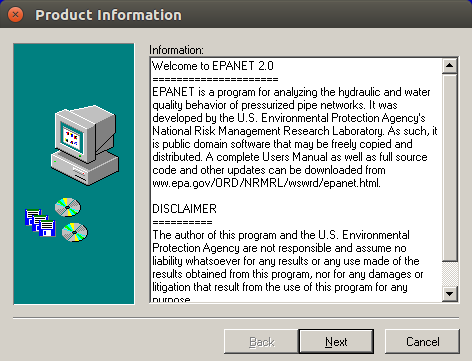
\includegraphics[scale=.3]{imatges/epanet/inst/1.png}
		\end{figure}
		\item Elegir el directori d'instal·lació (típicament C:$\backslash$Program Files)
		\begin{figure}[h!]
			\centering
			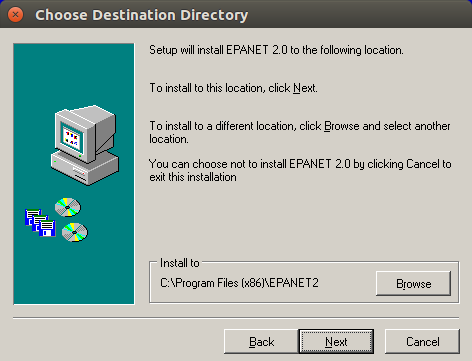
\includegraphics[scale=.3]{imatges/epanet/inst/2.png}
		\end{figure}
		\clearpage\item Finalitzar la instal·lació.
		\begin{figure}[h!]
			\centering
			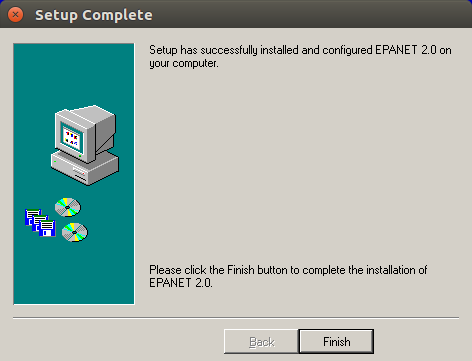
\includegraphics[scale=.3]{imatges/epanet/inst/3.png}
		\end{figure}
		\item Iniciar el programa.
		\begin{figure}[h!]
			\centering
			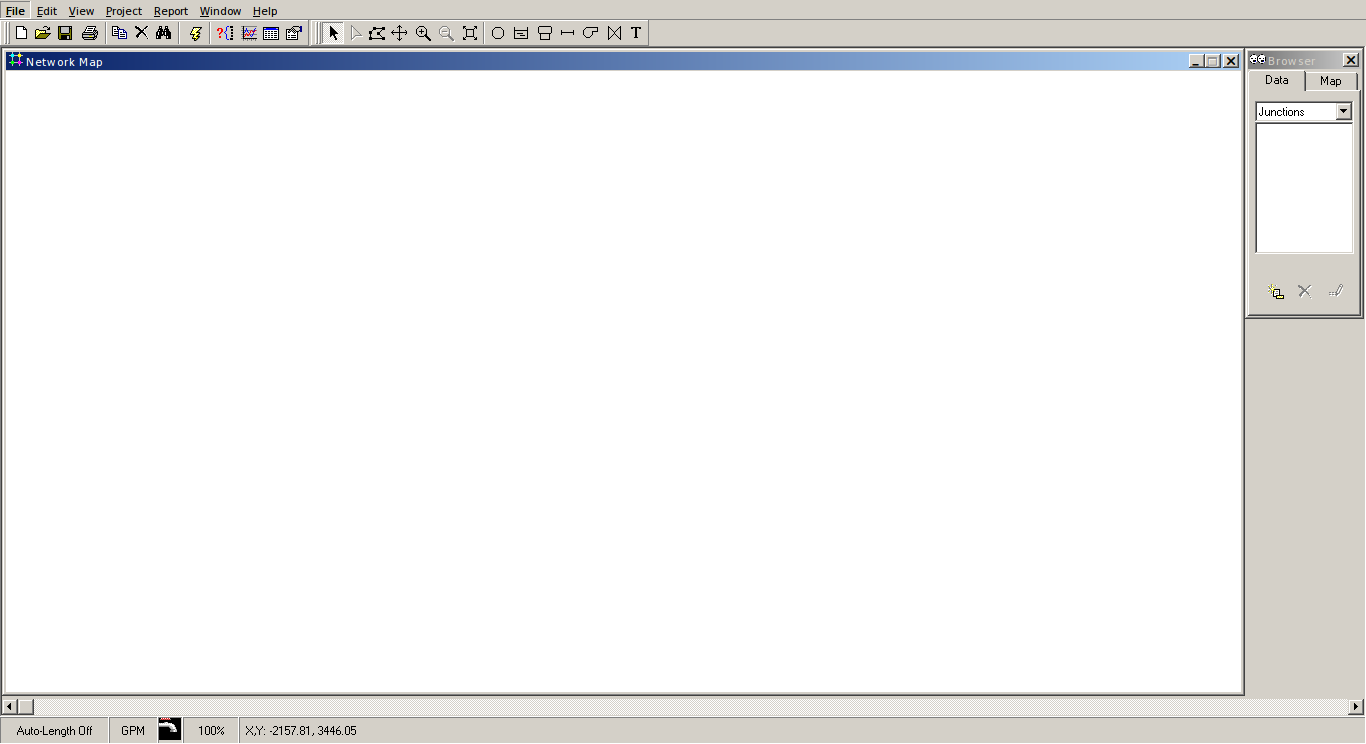
\includegraphics[scale=.15]{imatges/epanet/inst/4.png}
		\end{figure}
	\end{itemize}
\end{enumerate}

\subsection{Configuració bàsica de l'entorn}
El primer que cal fer per crear una xarxa utilitzant l'eina EPANET és configurar el \textit{layout} del projecte perquè treballi amb les unitats del sistema internacional (litres, metres, segons, etc).
\\\\Per això cal anar a \path{Menu/Projects/Defaults} i en la pestanya \textit{Hydraulics} establir les unitats de flux a LPS (Litros por segundo).
\begin{figure}[h!]
	\centering
	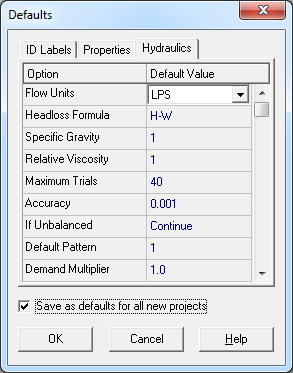
\includegraphics[scale=.7]{imatges/epanet/1.png}
	\caption{Establir les unitats del sistema internacional.}
\end{figure}
\\\\La representació gràfica dels components es pot modificar des de \path{Menu/View/Options}
\begin{figure}[h!]
	\centering
	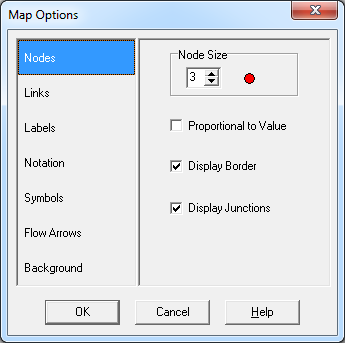
\includegraphics[scale=.7]{imatges/epanet/2.png}
	\caption{Configuració de les propietats dels components gràfics.}
\end{figure}
\\\\El límit de coordenades (marge inferior esquerra i el marge superior dret) es pot configurar des del menú \path{Menu/View/Dimensions}

\clearpage
\subsection{Implementació d'una nova xarxa de distribució (Exemple.net)\label{xarxaEPANET}}
En aquest apartat es mostrarà un exemple bàsic de creació d'una xarxa de distribució d'aigua.
\subsubsection{Eines}
Per crear una nova xarxa s'utilitzen els components de la barra d'eines del planol\footnote{Si aquesta barra d'eines no està visible es pot activar des de \path{Menu/View/Toolbars/Map}}.
\begin{figure}[h!]
	\centering
	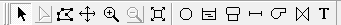
\includegraphics[scale=1]{imatges/epanet/4.png}
	\caption{Eines disponibles per la creació de xarxes.}
\end{figure}
Algunes de les eines més importants són
\begin{itemize}
	\item[] 
\includegraphics{imatges/epanet/4_1.png} Tanc.
	\item[] 
\includegraphics{imatges/epanet/4_2.png} Nus.
	\item[] 
\includegraphics{imatges/epanet/4_3.png} Sortidor.
	\item[] 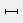
\includegraphics{imatges/epanet/4_4.png} Canonada.
	\item[] 
\includegraphics{imatges/epanet/4_5.png} Bomba d'aigua.
	\item[] 
\includegraphics{imatges/epanet/4_6.png} Vàlvula.
\end{itemize}

\subsubsection{Disseny}
En primer lloc repartim els componen que composen la xarxa, en aquest cas disposem de:
\begin{itemize}
	\item 1 diposit (1)
	\item 8 nodes (2-9)
	\item 1 tanc (10)
	\item 1 Bomba (8)
	\item 2 Vàlvules (10-11)
\end{itemize}
Aquesta representació quedarà de la següent manera.
\begin{figure}[h!]
	\centering
	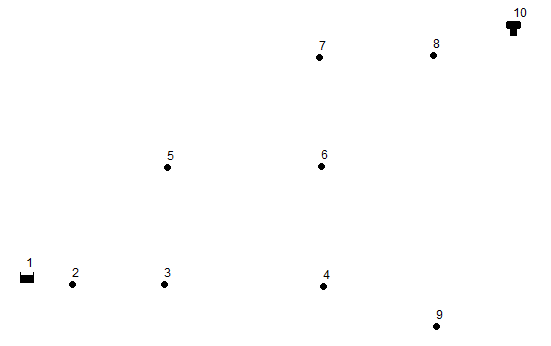
\includegraphics[scale=.7]{imatges/epanet/5.png}
	\caption{Diagrama sense connexions.}
\end{figure}
\\\\Ara toca connectar els components a través de canonades, per això, fem les següents connexions 1-2, 3-4, 4-9, 3-5, 5-6, 5-7\footnote{Com que aquesta connexió no és recta, cal resseguir el camí per representar la corba de la canonada.}, 6-7, 4-6. 
\\\\Tot seguit connectem els nodes 2-3 amb una bomba i els nodes 4-9 i 7-8 amb una vàlvula.
\\\\L'estructura de la xarxa hauria de ser similar a la de la següent imatge
\pagebreak
\begin{figure}[h!]
	\centering
	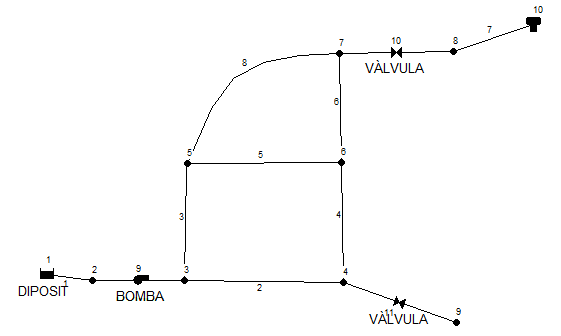
\includegraphics[scale=.6]{imatges/epanet/6.png}
	\caption{Diagrama amb connexions.}
\end{figure}
Un cop es té la distribució dels components, cal assignar les propietats que caracteritzen a cada component, per això s'ha de fer doble clic sobre el component i canviar els seus valors.
\\\\Per aquest exemple canviarem les següents propietats: 
\begin{figure}[h!]
	\centering
	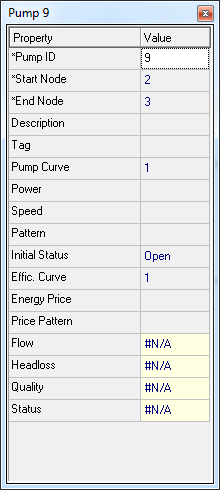
\includegraphics[scale=0.35]{imatges/epanet/car/bomba.png}
	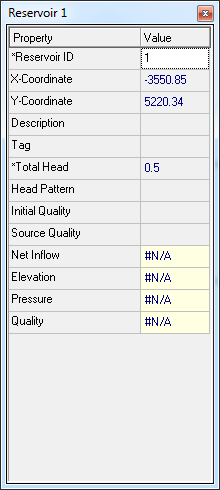
\includegraphics[scale=0.35]{imatges/epanet/car/diposit.png}
	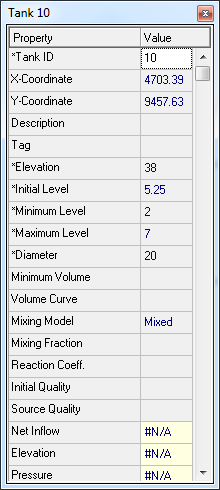
\includegraphics[scale=0.35]{imatges/epanet/car/sortidor.png}
	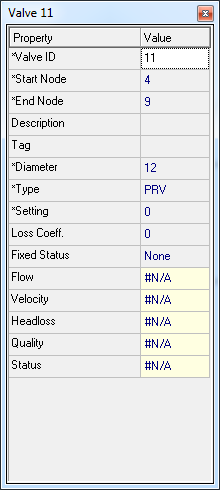
\includegraphics[scale=0.35]{imatges/epanet/car/valvula.png}
	\caption{Bomba, diposit, sortidor i valvula}
\end{figure}

\pagebreak
Per crear la configuració de la corba característica de la bomba, seleccionem \say{curve} del desplegable del \say{browser} i creem una nova corba.
\begin{figure}[h!]
	\centering
	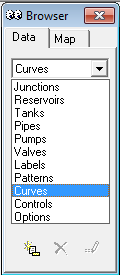
\includegraphics[scale=0.6]{imatges/epanet/10.png}
	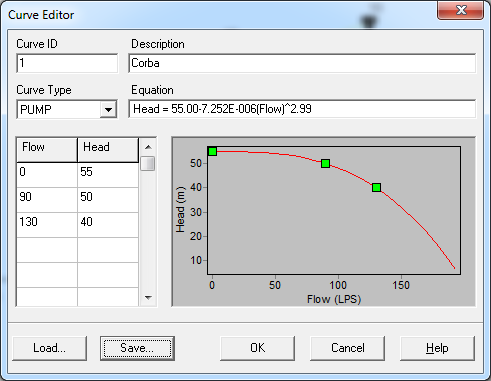
\includegraphics[scale=0.4]{imatges/epanet/11.png}
	\caption{Creació d'una nova corba.}
\end{figure}

\clearpage
\subsection{Anàlisi simple (Net3.net)}
Un cop s'ha modelat la xarxa, es pot realitzar una anàlisi hidràulic de règim permanent\footnote{Les necessitats dels diferents nusos no varien en funció del temps}. El primer que farem és guardar el model\footnote{El format d'emmagatzemament per defecte dels projectes és binari (.net).}, seguidament, per executar-lo cal fer clic al botó \path{Menu/Project/Run Analisys}. 
\\\\Si tot ha anat bé i el model és correcte, hauria de sortir la següent finestra informativa.
\begin{figure}[h!]
	\centering
	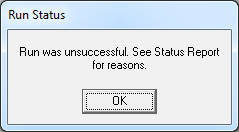
\includegraphics[scale=.5]{imatges/epanet/12.png}
	\caption{Execució correcte.}
\end{figure}
\\\\Aquesta acció genera diferents resultats accessibles des de \path{Menu/Report}. Alguns d'aquests resultats són:
\subsubsection{Status report}
S'hi pot accedir des de \path{Menu/Report/Status} i conté el log de tots els events generats durant la simulació. El resultat per aquesta simulació es pot veure en l'\textbf{annex \ref{ann2}}.

\subsubsection{Energy report}
S'hi pot accedir des de \path{Menu/Report/Energy} i conté una taula amb el comportament de les bombes en la simulació.
\begin{figure}[h!]
	\centering
	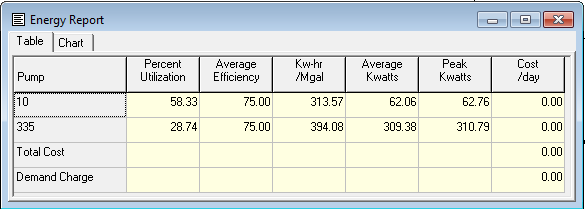
\includegraphics[scale=.5]{imatges/epanet/reports/energia.png}
	\caption{Taula d'energia de les bombes.}
\end{figure}

\subsubsection{Balanç}
S'hi pot accedir des de \path{Menu/Report/Graph} seleccionant \textit{System Flow} com a tipus de graf.
\begin{figure}[h!]
	\centering
	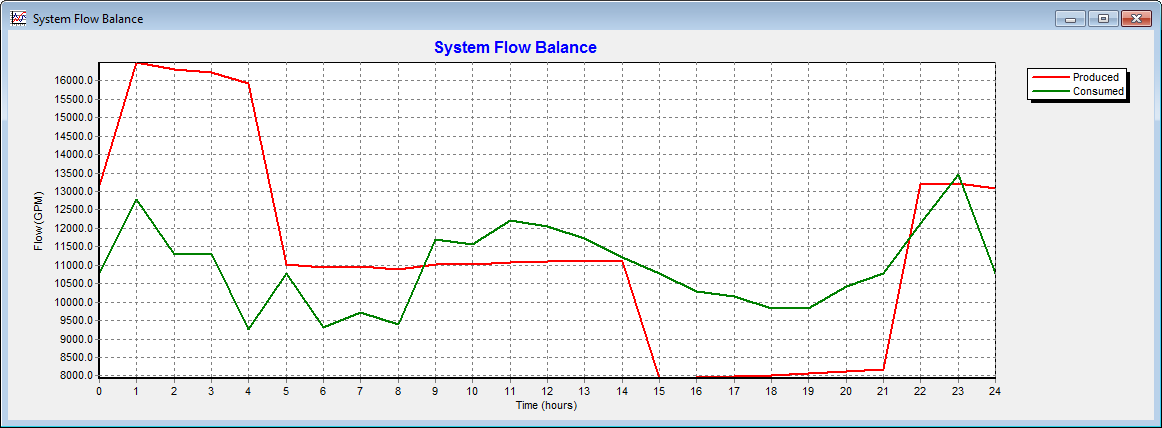
\includegraphics[scale=.5]{imatges/epanet/reports/balans.png}
	\caption{Balanç de la demanda.}
\end{figure}

\subsubsection{Taula de resultats}
S'hi pot accedir des de \path{Menu/Report/Table} i conté una taula amb el valor dels paràmetres indicats en funció del temps.
\begin{figure}[h!]
	\centering
	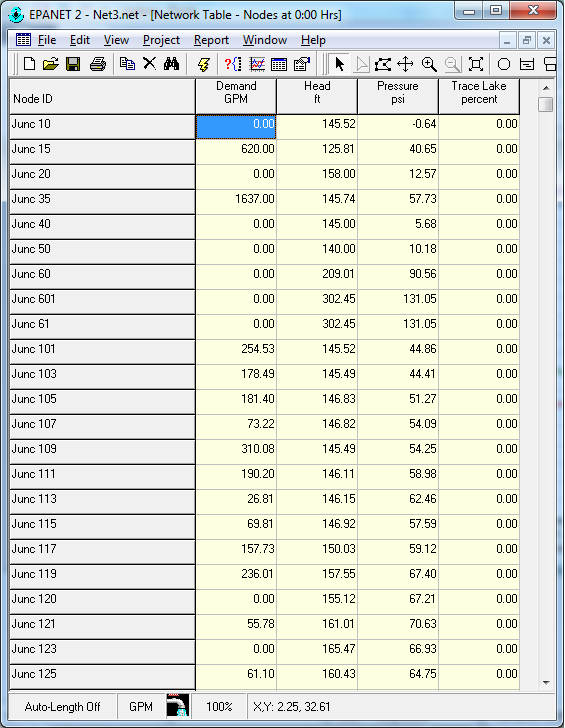
\includegraphics[scale=.5]{imatges/epanet/reports/taula.png}
	\caption{Taula de resultats de l'execució.}
\end{figure}

\pagebreak
\subsubsection{Full report}
S'hi pot accedir des de \path{Menu/Report/Full} i genera un fitxer \textit{.rep} que es pot obrir amb altres eines com el \textit{Crystal reports viewer}\cite{crystalReports} de \textit{SAP} per interpretar el seu contingut.


\pagebreak
\subsection{Període variant}
Per fer el model més realista, es pot adaptar perquè la demanda dels nodes variï en funció del temps, això es farà gràcies a un patró que assignarem com a corba de modulació. 
\\\\Per posar un exemple, configurarem la xarxa de tal manera que la simulació tingui una durada de 72 hores i que el patró dels components canviï cada hora. Per a establir aquesta configuració s'ha de seleccionar l'opció \path{Browser/Options/Time} i assignar un valor de 72 a la variable \textit{Total duration} i un valor d'1 a la variable \textit{Pattern time step}.
\begin{figure}[h!]
	\centering
	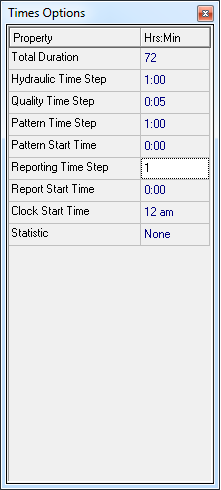
\includegraphics[scale=.7]{imatges/epanet/15.png}
	\caption{Configuració dels intervals de temps.}
\end{figure}
\\\\Un cop tenim configurada la freqüència de variació, cal configurar el grau de demanda a cada interval, per fer això cal crear patrons i això es pot fer des de \path{Browser/Options/Patterns}. 
\pagebreak
\begin{figure}
	\centering
	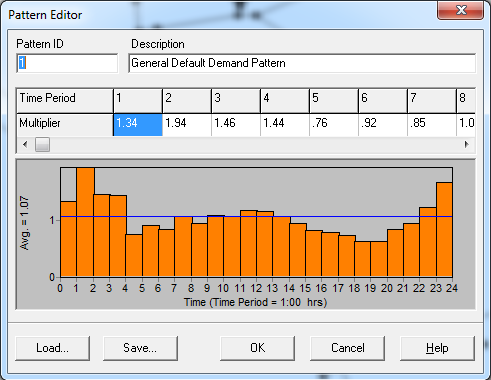
\includegraphics[scale=.5]{imatges/epanet/16.png}
	\caption{Configuració del patró pel temps.}
\end{figure}
\\\\Un cop es té creat el patró, s'ha d'assignar com a corba de modulació, per a fer això hi ha dues opcions:
\begin{itemize}
	\item Configurar cada node amb el patró.
\begin{figure}[h!]
	\centering
	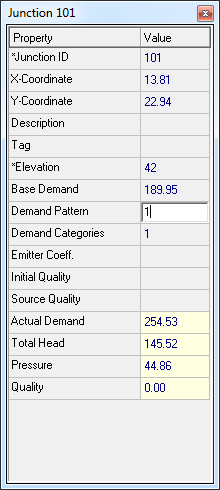
\includegraphics[scale=.5]{imatges/epanet/18.png}
	\caption{Configuració d'un node}
	\label{fig:confNodeAnode}
\end{figure}
	\item Establir una configuració global per tots els nodes des de \path{Menu/Porject/Defaults.../Hydraulics}. Aquesta configuració només és possible si es disposa d'un únic patró.
\end{itemize}
\begin{figure}[h!]
	\centering
	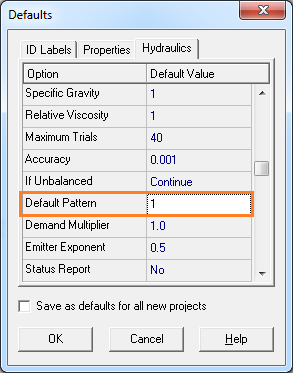
\includegraphics[scale=.5]{imatges/epanet/19.png}
	\caption{Configuració global}
	\label{fig:confGlobal}
\end{figure}
Configurada la xarxa, es pot executar i obtenir uns resultats, on aquest cop, variarant les propietats dels components en funció del temps.

\clearpage
\subsection{Propietats}
En aquest apartat es descriuen algunes de les propietats del programa.

\subsubsection{Algorismes utilitzats en l'anàlisi}
En el manual d'usuari\cite{DocuEpanet} es descriuen detalladament els algorismes utilitzats en l'informe de resultats de la qualitat de l'aigua.

\subsubsection{Format dels fitxers d'exportació}
Els fitxers d'exportació que es generen des de \textit{EPANET} i que llavors podem importar a altres eines, estan definits per un seguit de capçaleres i les seves propietats, on cada capçalera correspon a un component representable. En la següent imatge es llisten els components disponibles.
\begin{figure}[h!]
	\centering
	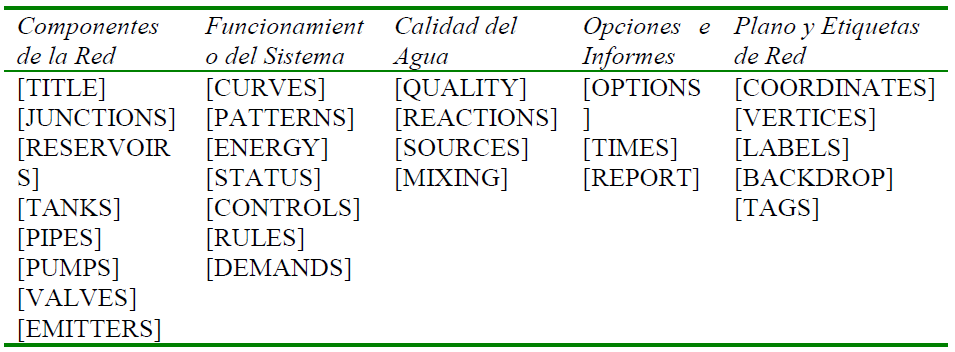
\includegraphics[scale=.5]{imatges/epanet/components.png}
	\caption{Representació dels components d'EPANET}
\end{figure}
\\\\Per exemple, per exportar la xarxa desenvolupada en la secció \ref{xarxaEPANET} (Exemple.net) s'ha d'accedir a \path{Menu/Expor/Map} i seleccionar el format que volem exportar, en aquest cas exportarem la xarxa sencera, i per això, seleccionem \textit{Network...} i li assignem un nom. Això generarà un fitxer amb extensió \textit{.inp} que inclou totes les propietats de la xarxa.
\\\\El contingut de l'arxiu per aquesta xarxa es pot veure en \textbf{l'annex \ref{ann1}.}

\subsubsection{Interpretació dels errors}
En el moment d'executar la simulació, es poden produir diversos errors en l'anàlisi, alguns exemples són:
\begin{itemize}
	\item \textbf{error 101}: Anàlisi interromput per falta de memòria.
	\item \textbf{error 110}: Anàlisi interromput degut a que les equacions hidràuliques establertes no es poden resoldre.
	\item \textbf{error 202}: Valor numèric il·legal assignat a una propietat.
\end{itemize}
El llistat complet dels errors es pot consultar en l'annex B del manual d'usuari\cite{DocuEpanet}.

\clearpage
\subsection{Altres exemples}
Alguns exemples de models de xarxes extrets d'Internet.
\begin{figure}[h!]
	\centering
	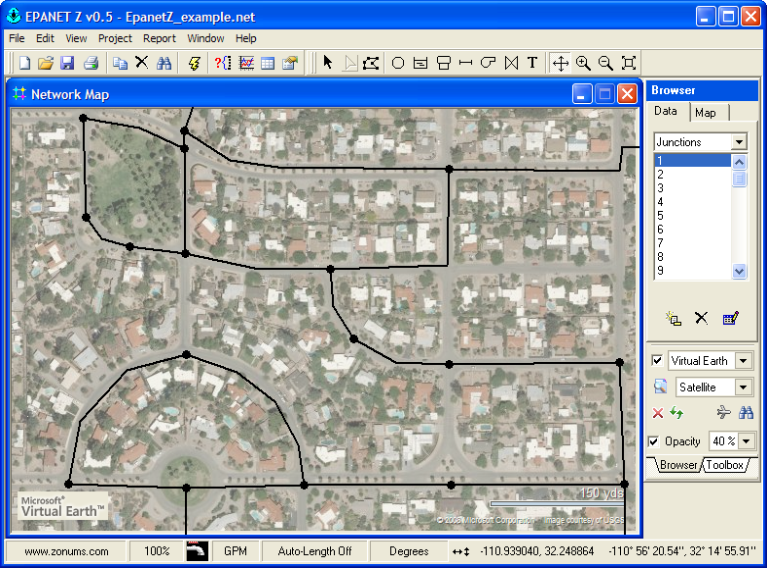
\includegraphics[width=65mm, height=50mm]{imatges/epanet/exemples/x1.png}
	\hspace{.2cm}
	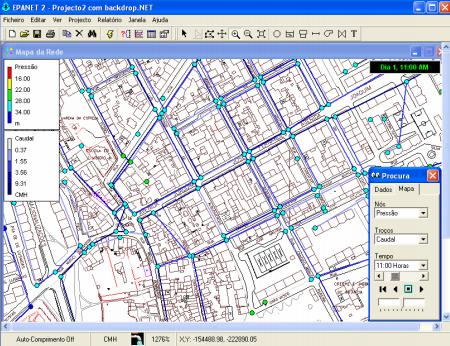
\includegraphics[width=65mm, height=50mm]{imatges/epanet/exemples/x2.jpg}
	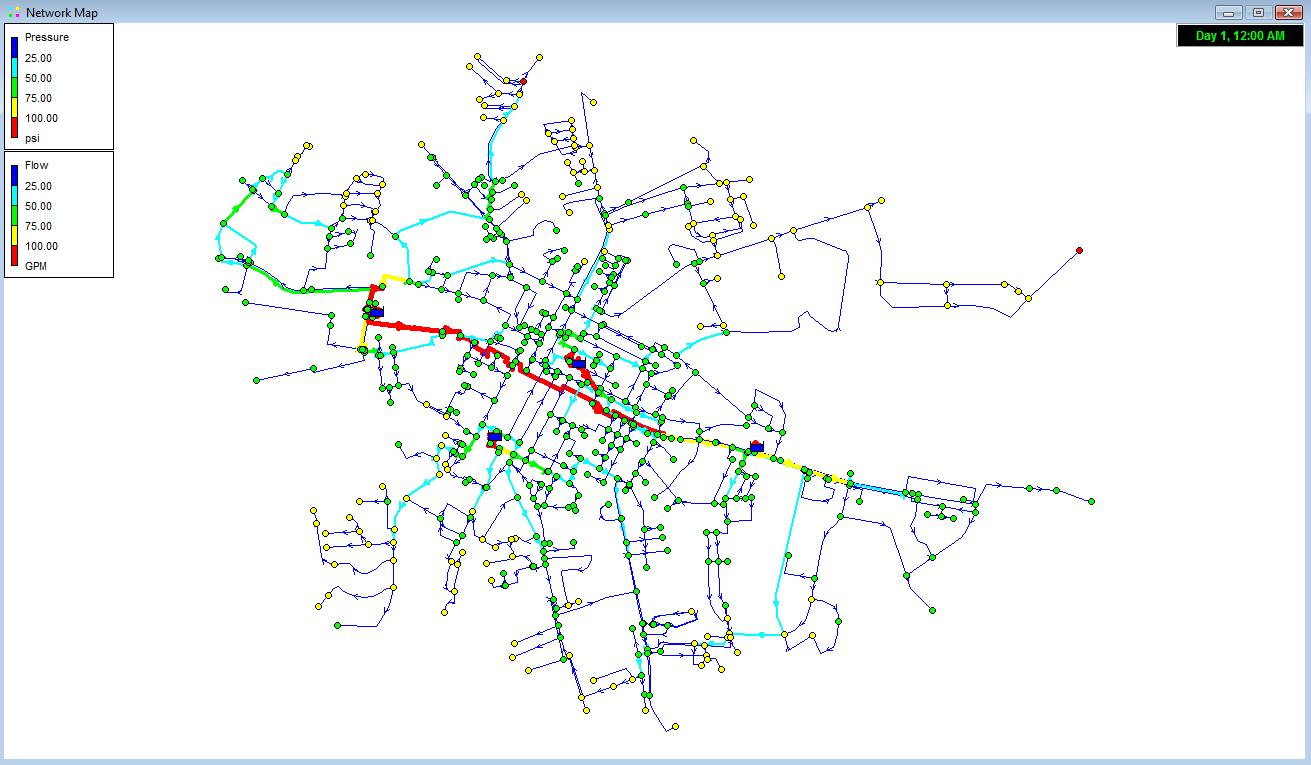
\includegraphics[width=65mm, height=50mm]{imatges/epanet/exemples/x3.jpg}
	\hspace{.2cm}
	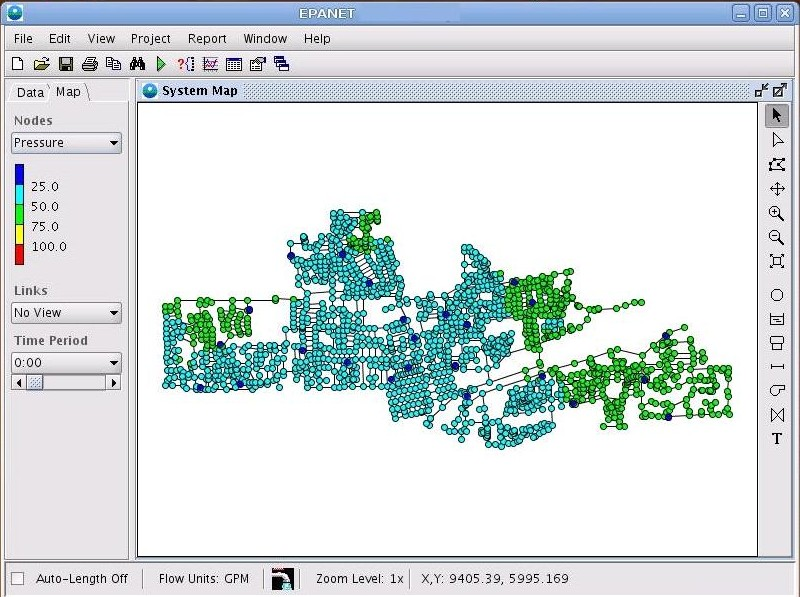
\includegraphics[width=65mm, height=50mm]{imatges/epanet/exemples/x4.jpg}
	\caption{Exemple de xarxes extretes d'Internet.}
\end{figure}
\subsection{Conclusió d'EPANET}
L'eina EPANET és intuïtiva i senzilla d'utilitzar, pot carregar models que estan en diferents formats, i de cara al problema plantejat en la secció \ref{problema} pot ser útil a l'hora de modelar la xarxa que s'ha d'analitzar.



%%%%%%%%%%%%%%%TEVA-SPOT%%%%%%%%%%%%%%%%%
\clearpage
\section{TEVA-SPOT Toolkit\label{teva-spoot}}
En aquesta secció es mostra com es pot modelar un problema de posicionament de sensors sobre una xarxa de distribució d'aigua, utilitzat l'eina TEVA-SPOT.
\\\\\textbf{És important assegurar que el model a utilitzar s'executa correctament utilitzant l'eina \textit{EPANET}.}
\subsection{Instal·lació}
Aquesta eina disposa d'una línea de comandes i d'una interficie gràfica, segons les necessitats de cada usuari es pot utilitzar una versió del programa o una altre.

\subsubsection{Linia de comandes}
Descarregar els binaris del programa \cite{tevaSpotExec}.

\subsubsection{Interfície gràfica}
L'eina TEVA-SPOT Toolkit també disposa d'una interfície gràfica\cite{tevaSpotGui} per facilitar i agilitzar la seva utilització. En aquest document i en la mesura que sigui possible, s'utilitzarà aquesta eina.
\\\\Per poder utilitzar-la, cal disposar de:
\begin{itemize}
	\item Java Developement Kit (JDK) 1.6 actualització 20 o superior.
	\item Python 2.6 o superior.
\end{itemize}
\textbf{Aquestes dependències, cal que estiguin instal·lades abans de començar la instal·lació de TEVA-SPOT.}

\subsection{Metodologia de posicionament de sensors}
Hi ha diferentes metodologies per resoldre el problema del posicionament de sensors\footnote{Metodologies basades en l'opinió d'experts, mètodes de ranking, optimització, etc.}, la metodologia utilitzada per TEVA-SPOT Toolkit és l'optimització on l'objectiu és trobar una configuració de sensors que minimitzi el risc dels contaminants.

\subsection{Estructura de dades}
L'estructura de dades que utilitza TEVA-SPOT és jeràrquica, i es pot representar en el següent esquema.
\begin{figure}[h!]
	\centering
	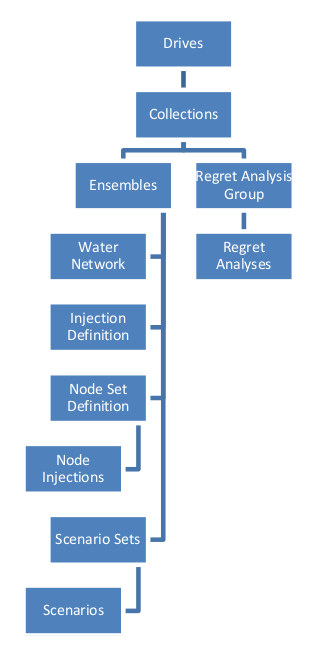
\includegraphics[scale=.5]{imatges/teva-spot/esquema.png}
	\caption{Estructura de dades de TEVA-SPOT.}
\end{figure}
\\\\TEVA-SPOT té dos modes de treball.
\begin{itemize}
	\item \textit{Ensamble analysis mode:} és el mode a utilitzar per fer l'anàlisi de vulnerabilitat dels contaminants i el disseny de la xarxa de sensors.
	\item \textit{Regret analysis mode:} és el mode a utilitar per analitzar la xarxa de sensors. 
\end{itemize}
\subsection{Exemple}
Per veure el funcionament d'aquesta eina, s'analitzarà una de les xarxes que ja ve com a exemple amb el programa. Aquesta xarxa és la \textit{Net3} i compta amb 97 nodes.
\\\\En aquesta secció es seguiran 5 passos.
\begin{enumerate}
	\item Definir l'estructura del projecte.
	\item Simulació d'incidents contaminants.
	\item Computar l'impacte dels contaminants.
	\item Posicionament de sensors.
	\item Evaluar el posicionament de sensors.
\end{enumerate}

\subsubsection{Definir l'estructura del projecte}
El primer que cal fer per començar a treballar amb TEVA-SPOT és definir un ensamblat, per això cal anar a 

\subsubsection{Simulació d'incidents contaminants}

\subsubsection{Computar l'impacte dels contaminants}

\subsubsection{Posicionament de sensors}

\subsubsection{Evaluar el posicionament de sensors}

\clearpage
\section{Versions utilitzades}
Les versions dels programes que s'han utilitzat per desenvolupar aquest projecte són:
\begin{itemize}
	\item EPANET 2.00.12
	\item TEVA-SPOT 2.3.2-MSX Beta 20170110
	\item JDK 1.8.0\_111 (Oracle Corporation)
	\item Python 2.7.14
\end{itemize}

%%%%%%%%%%%%%%%DOCUMENTACIÓ%%%%%%%%%%%%%%%%%
\clearpage
\section{Documentació utilitzada}
La documentació disponible i que s'ha seguit per elaborar aquest manual és:
\begin{itemize}
	\item Manual d'usuari d'EPANET (\path{/docs/EPANET.pdf)}.
	\item Manual d'usuari del TEVA-SPOT Toolkit (\path{/docs/TEVA-SPOT.pdf}).
	\begin{itemize}
		\item Introducció.
		\item Utilització bàsica.
		\item Formulació a utilitzar per presentar un problema de posicionament de sensors.
		\item Incidents contaminants i impacte de les mesures.
		\item Solvers disponibles.
		\item Format de les dades.
	\end{itemize}
	\item Manual d'usuari per utilitzar la interfície gràfica de TEVA-SPOT Toolkit (\path{/docs/TEVA-SPOT-GUI.pdf}).
\end{itemize}




%%%%%%%%%%%%%%%BIBLIOGRAFIA%%%%%%%%%%%%%%%%%
\clearpage
\begin{thebibliography}{9}
	\bibitem{epanet}\textit{EPANET}:
  	\\\path{https://www.epa.gov/water-research/epanet}
  	
  	\bibitem{DocuEpanet}\textit{Documentació EPANET}:
  	\\\path{http://epanet.info/manuales/}
  	
	\bibitem{tevaSpot}\textit{TEVA-SPOT}:
  	\\\path{https://software.sandia.gov/trac/spot/wiki}

  	\bibitem{tevaSpotExec}\textit{TEVA-SPOT EXECUTABLE}:
  	\\\path{https://software.sandia.gov/trac/spot/downloader}

	\bibitem{tevaSpotGui}\textit{TEVA-SPOT Interfície gràfica}:
  	\\\path{https://cfpub.epa.gov/si/si_public_record_report.cfm?subject=Homeland\%20Security\%20Research&dirEntryId=257684}
  	
	\bibitem{crystalReports}\textit{Crystal Reports Viewer}:
  	\\\path{www.crystalreports.com/crystal-viewer}
\end{thebibliography}

\clearpage
\begin{appendices}
\section{Xarxa 1\label{ann1}}
En aquest annex es mostra el contingut del fitxer per la xarxa desenvolupada en aquest document.\footnote{Aquest mateix fitxer es pot trobar en \path{/xarxes/primera.inp}}
\lstinputlisting[language={}]{xarxes/exportades/x1.inp}

\section{Report d'estat de la xarxa\label{ann2}}
En aquest annex es mostra el contingut del fitxer generat per epanet de l'estat de la xarxa durant la simulació.
\lstinputlisting[language={}]{xarxes/reports/Net3_status.txt}
\end{appendices}
\end{document}